% ######### DOCUMENT SETUP

\documentclass[a4paper,twoside,openright,makeidx,12pt]{book}
\usepackage{draftcopy}
%% Faire un checkout sur le module TeX-tools pour obtenir les fichiers partag�s
%$Id: macro.tex,v 1.10 2004/12/08 13:38:58 acary Exp $


%\usepackage{a4wide}
\textheight 25cm
\textwidth 16.5cm
\topmargin -1cm
%\evensidemargin 0cm
\oddsidemargin 0cm
\evensidemargin0cm
\usepackage{layout}


\usepackage{amsmath}
\usepackage{amssymb}
\usepackage{minitoc}
%\usepackage{glosstex}
\usepackage{colortbl}
\usepackage{hhline}
\usepackage{longtable}

%\usepackage{glosstex}
%\def\glossaryname{Glossary of Notation}
\def\listacronymname{Acronyms}

\usepackage[outerbars]{changebar}\setcounter{changebargrey}{20}
%\glxitemorderdefault{acr}{l}

%\usepackage{color}
\usepackage{graphicx,epsfig}
\graphicspath{{./Figures/}}
\usepackage[T1]{fontenc}
\usepackage{rotating}

%\usepackage{algorithmic}
%\usepackage{algorithm}
\usepackage{ntheorem}
\usepackage{natbib}


%\renewcommand{\baselinestretch}{2.0}
\setcounter{tocdepth}{2}     % Dans la table des matieres
\setcounter{secnumdepth}{3}  % Avec un numero.



\newtheorem{definition}{Definition}
\newtheorem{lemma}{Lemma}
\newtheorem{claim}{Claim}
\newtheorem{remark}{Remark}
\newtheorem{assumption}{Assumption}
\newtheorem{example}{Example}
\newtheorem{conjecture}{Conjecture}
\newtheorem{corollary}{Corollary}
\newtheorem{OP}{OP}
\newtheorem{problem}{Problem}
\newtheorem{theorem}{Theorem}


\newcommand{\CC}{\mbox{\rm $~\vrule height6.6pt width0.5pt depth0.25pt\!\!$C}}
\newcommand{\ZZ}{\mbox{\rm \lower0.3pt\hbox{$\angle\!\!\!$}Z}}
\newcommand{\RR}{\mbox{\rm $I\!\!R$}}
\newcommand{\HH}{\mbox{\rm $I\!\!H$}}
\newcommand{\NN}{\mbox{\rm $I\!\!N$}}

\newcommand{\Mnn}{\mathcal M^{n\times n}}
\newcommand{\Mnp}[2]{\ensuremath{\mathcal M^{#1\times #2}}}



\newcommand{\Frac}[2]{\displaystyle \frac{#1}{#2}}

\newcommand{\DP}[2]{\displaystyle \frac{\partial {#1}}{\partial {#2}}}

% c++ variables writting
\newcommand{\varcpp}[1]{\textit{#1}}
% itemize
\newcommand{\bei}{\begin{itemize}}
\newcommand{\ei}{\end{itemize}}

\newcommand{\ie}{i.e.}
\newcommand{\eg}{e.g.}
\newcommand{\cf}{c.f.}
\newcommand{\putidx}[1]{\index{#1}\textit{#1}}

\def\Er{{\rm I\! R}}
\def\En{{\rm I\! N}} 
\def\Ec{{\rm I\! C}}
 
\def\zc{\hat{z}}
\def\wc{\hat{w}}

\font\tete=cmr8 at 8 pt


% normal tangent
\def\n{{\hbox{\tiny{N}}}}
\def\t{{\hbox{\tiny{T}}}}
\def\nt{\hbox{\tiny{NT}}}
\def\nsf{\hbox{\tiny{\textsf N}}}
\def\tsf{\hbox{\tiny{\textsf T}}}
\def\sigman{\sigma_{\n}}
\def\sigmat{\sigma_{\t}}
\def\sigmant{\sigma_{\nt}}
\def\epsn{\epsilon_{\n}}
\def\epst{\epsilon_{\t}}
\def\epsnt{\epsilon_{\nt}}
\def\eps{\epsilon}
\def\veps{\varepsilon}
\def\sig{\sigma}
\def\Rn{R_{\n}}
\def\Rt{R_{\t}}
\def\cn{c_{\n}}
\def\Cn{C_{\n}}
\def\ct{c_{\t}}
\def\Ct{C_{\t}}
\def\un{u_{\n}}
\def\ut{\buu_{\t}}
\def\uut{u_{\t}}
\def\unc{u_{\n}^c}
\def\utc{\buu_{\t}^c}
\def\vn{v_{\n}}
\def\vt{v_{\t}}
\def\rr{\hbox{\tiny{\textsf R}}}
\def\irr{\hbox{\tiny{\textsf{IR}}}}
\def\rn{r_{\n}}
\def\rt{\brr_{\t}}
\def\rnc{r_{\n}^c}
\def\rtc{\brr_{\t}^c}
\def\trn{\Tilde{r}_{\n}}
\def\trt{\Tilde{\brr}_{\t}}
\def\tr{\Tilde{\brr}}
\def\tv{\Tilde{\bvv}}
\def\vn{v_{\n}}
\def\vt{\bvv_{\t}}
\def\adh{\mathsf{adh}}
\def\adj{\hbox{\tiny{\textsf{adj}}}}
\def\adjc{\hbox{\tiny{\textsf{adjC}}}}
\def\adja{\hbox{\tiny{\textsf{adjA}}}}
\def\cc{\hbox{\tiny{\textsf C}}}
\def\ca{\hbox{\tiny{\textsf A}}}

\DeclareMathOperator{\proj}{proj}
\DeclareMathOperator{\expm}{expm}
\DeclareMathOperator{\dexp}{dexp}
\DeclareMathOperator{\dlexp}{d^l exp}
\DeclareMathOperator{\drexp}{d^r exp}
\DeclareMathOperator{\dexpm}{dexpm}
\DeclareMathOperator{\expq}{expq}
\DeclareMathOperator{\dexpq}{dexpq}
\DeclareMathOperator{\Ad}{Ad}
\DeclareMathOperator{\ad}{ad}
\DeclareMathOperator{\dd}{d}



%%  Les ensembles de nombres  C. Fiorio (fiorioÊatÊmath.tu-berlin.de) 
%
\def\nbR{\ensuremath{\mathrm{I\!R}}} % IR
\def\nbN{\ensuremath{\mathrm{I\!N}}} % IN
\def\nbF{\ensuremath{\mathrm{I\!F}}} % IF
\def\nbH{\ensuremath{\mathrm{I\!H}}} % IH
\def\nbK{\ensuremath{\mathrm{I\!K}}} % IK
\def\nbL{\ensuremath{\mathrm{I\!L}}} % IL
\def\nbM{\ensuremath{\mathrm{I\!M}}} % IM
\def\nbP{\ensuremath{\mathrm{I\!P}}} % IP

%----------------------------------------------------------------------
%                  Modification des subsubsections
%----------------------------------------------------------------------
\makeatletter
\renewcommand\thesubsubsection{\thesubsection.\@alph\c@subsubsection}
\makeatother

%----------------------------------------------------------------------
%             Redaction note environnement
%----------------------------------------------------------------------
\makeatletter
\theoremheaderfont{\scshape}
\theoremstyle{marginbreak}
\theorembodyfont{\upshape}
%\newtheorem{rque}{\bf Remarque}[chapter]
%\newtheorem{rque1}{\bf \fsc{Remarque}}[chapter] !!! \fsc est une commande french
\newtheorem{ndr1}{\textbf{\textsc{Redaction note}}}[section]

\newenvironment{ndr}%
{%
\tt
%\centerline{---oOo---}
\noindent\begin{ndr1}%
}%
{%
\begin{flushright}%
%\vspace{-1.5em}\ding{111}
\end{flushright}%
\end{ndr1}%
%\centerline{---oOo---}
}

\makeatother

%----------------------------------------------------------------------
%             Redaction note environnement V.ACARY
%----------------------------------------------------------------------
\makeatletter
\theoremheaderfont{\scshape}
\theoremstyle{marginbreak}
\theorembodyfont{\upshape}
%\newtheorem{rque}{\bf Remarque}[chapter]
%\newtheorem{rque1}{\bf \fsc{Remarque}}[chapter] !!! \fsc est une commande french
\newtheorem{ndr1va}{\textbf{\textsc{Redaction note V. ACARY}}}[section]

\newenvironment{ndrva}%
{%
\tt
%\centerline{---oOo---}
\noindent\begin{ndr1va}%
}%
{%
\begin{flushright}%
%\vspace{-1.5em}\ding{111}
\end{flushright}%
\end{ndr1va}%
%\centerline{---oOo---}
}

\makeatother
%----------------------------------------------------------------------
%             Redaction note environnement V.ACARY
%----------------------------------------------------------------------
\makeatletter
\theoremheaderfont{\scshape}
\theoremstyle{marginbreak}
\theorembodyfont{\upshape}
%\newtheorem{rque}{\bf Remarque}[chapter]
%\newtheorem{rque1}{\bf \fsc{Remarque}}[chapter] !!! \fsc est une commande french
\newtheorem{ndr1fp}{\textbf{\textsc{Redaction note F. PERIGNON}}}[section]

\newenvironment{ndrfp}%
{%
\tt
%\centerline{---oOo---}
\noindent\begin{ndr1fp}%
}%
{%
\begin{flushright}%
%\vspace{-1.5em}\ding{111}
\end{flushright}%
\end{ndr1fp}%
%\centerline{---oOo---}
}

\makeatother
%----------------------------------------------------------------------
%                  Chapter head enviroment
%----------------------------------------------------------------------
\newenvironment{chapter_head}
{%
\begin{center}%
-------------------- oOo --------------------\\%
\ \\%
\begin{minipage}[]{14cm}%
\noindent\normalsize\advance\baselineskip-1pt %
}%
{%
\par\end{minipage}%
\ \\%
\ \\%
-------------------- oOo --------------------
\end{center}%
\vspace*{\stretch{1}}%
\clearpage%
\thispagestyle{empty}%
\vspace*{\stretch{1}}%
\minitoc%
\vspace*{\stretch{2}}%
\clearpage%
}


\newcommand{\contract}{{\,:\,}}

%%% Local Variables: 
%%% mode: latex
%%% TeX-master: "report"
%%% End: 


\usepackage{fancyheadings} 
\usepackage{lastpage}

\pagestyle{fancy} 
\renewcommand{\chaptermark}[1]% 
{\markboth{{Chap-- \thechapter.\ #1}}{}} 
\renewcommand{\sectionmark}[1]% 
{\markright{{\thesection.\ #1}}} 
\setlength{\headrulewidth}{0.5pt} 
\setlength{\footrulewidth}{0.5pt} 
\newcommand{\helv}{% 
  \fontfamily{phv}\fontseries{b}\fontsize{9}{11}\selectfont} 
\lhead[\helv \thepage]{\helv \rightmark} 
\rhead[\helv \leftmark]{\helv \thepage} 
\cfoot{\acs{esd} -- November 17, 2004}

\makeindex

\begin{document}

\pagestyle{empty}
\renewcommand{\arraystretch}{1.8}
\thispagestyle{empty}

\begin{center}
\includegraphics[height=23mm, width=77mm]{figure/siconos.eps}\\
\textsf{European Project IST2001-37172}\\[6cm]
\end{center}

\begin{center}
\huge
\textsf{\textbf{\textit{External Specifications Document}}}\\[2.5cm]
\end{center}

\large
\begin{center}
\textsf{\textbf{Version :} 1.1}\\
\textsf{\textbf{Status :}  In progress}\\
\textsf{\textbf{Date :} December 27, 2004} \\ % February 15, 2004}\\
\textsf{\textbf{Document Code :} \acs{esd}}\\[5cm]

\end{center}

\normalsize

\begin{flushright}

\includegraphics[scale=0.3]{figure/Logo-INRIA.eps}
\end{flushright}

\clearpage




%\maketitle

%-----------------------------------------------------------------------------%

\normalsize

\begin{center}
  \textsf{\Large Identification}
\end{center}

\noindent\begin{tabular}{|p{0.3\textwidth}|p{0.7\textwidth}|}
\hline
Document Title : & \textsf{External Specifications Document} \\
Document Code :  & \textsf{\acs{esd}} \\
\hline
\end{tabular}
\textsf{ }\\


\begin{center}
  \textsf{\Large About the document and its author(s)}
\end{center}

\noindent\begin{tabular}{|p{0.3\textwidth}|p{0.7\textwidth}|}
\hline
Nature :& \textsf{This document aims to define the interface between the users and the platform.}\\
Language :& \textsf{English}\\
Author(s) :& \textsf{Jean-Michel Barbier, Vincent ACARY, Jean-Baptiste CHARLETY}\\
Possible remarks :& \textsf{}\\
References : &\textsf{\acs{esd}}\\
\hline
\end{tabular}

\textsf{ }\\

%\newpage

% % cartridge current version
% \renewcommand{\arraystretch}{1.1}
% \begin{center}
%   \textsf{\Large Current Version}
% \end{center}
% \begin{tabular}{|p{0.3\textwidth}|p{0.7\textwidth}|}
% \hline
% Date : &\textsf{November 17, 2004}\\
% Current version number : &\textsf{1.1}\\ 
% Status :&$\bigotimes$ in progress \\
% & $\bigcirc$ validated\\
% \textit{ }& \hspace{0.5cm} Approved by :\\
% \hline
% \end{tabular}

\renewcommand{\arraystretch}{1.2}
\begin{center}
  \textsf{\Large Current Version}
\end{center}
\begin{tabular}{|p{0.3\textwidth}|p{0.7\textwidth}|}
\hline
Date : &\textsf{November 17, 2004}\\
Current version number : &\textsf{1.1}\\ 
Status :&$\bigotimes$ in progress \\
& $\bigcirc$ validated\\
\textit{ }& \hspace{0.5cm} Approved by : \\
\hline
Document change record since last version : &
\begin{minipage}[t]{0.70\textwidth}
\textsf{User cases diagrams added} \\
\end{minipage}\\
\hline
\end{tabular}

\textsf{ }\\
\begin{center}
\textbf{Copyright Notice \copyright}\\
This document may not be reproduced (even partially) or communicated to third parties without the written authorisation of INRIA.
\end{center}
\renewcommand{\arraystretch}{1.8}


% log of changes  
\pagebreak
\begin{center}
  \textsf{\Large About the document developing process}
\end{center}
% \begin{tabular}{|p{0.3\textwidth}|p{0.7\textwidth}|}
% \hline
% Date of first issue : &\textsf{February 15, 2004}\\
% Current version number : &\textsf{1.0}\\ 
% Validated by :& \textsf{Vincent Acary}\\
% \hline
% Document change record since last version : &\textsf{First issue} \\
% \hline
% \hline
% Date of first issue : &\textsf{November 17, 2004}\\
% Current version number : &\textsf{1.1}\\ 
% Validated by :& \textsf{}\\
% \hline
% Document change record since last version : &\textsf{User cases added} \\
% \hline

% \end{tabular}
\begin{tabular}{|p{0.3\textwidth}|p{0.7\textwidth}|}
\hline
Date of first issue : &\textsf{15/02/2004}\\
\hline \hline
% ---
Version number : &\textsf{1.0}\\ 
Validated by :& \textsf{Vincent Acary}\\
Date : & \textsf{15/02/2004} \\
Document change record since last version : &\textsf{first issue} \\
\hline
% ---
% Version number : &\textsf{X.X}\\ 
% Validated by :& \textsf{}\\
% Date : & \textsf{dd/mm/yyyy} \\
% Document change record since last version : &\textsf{First issue} \\
% \hline
\end{tabular}

%\end{document}

%%%%%%%%%%%%%%%%%%%%%%%%%%%%%%%%%%%%%%%%%%%%%%%%%%%%%%%%%%%%%%%%%%%%%%%%%%%%%%%%%%%%%%%%%%%%%%%%%%%%%%%%%


\tableofcontents
\pagestyle{fancy}
\pagenumbering{arabic}


\cleardoublepage

% ######### TEXT


% ---------------------------------------------------------------------------------------%
% %
% CHAPTER                                                                                                                               %
% %
% ---------------------------------------------------------------------------------------%

\chapter{Using context}

% ---------------------------------------------------------------------------------------%
% section                                                                               %
% ---------------------------------------------------------------------------------------%
\section{Users}

For the first version of the \acs{siconos} software, most of the users are scientists from various scientific fields : mathematicians, physicists, electrical and mechanical   engineers\, etc. Their computer skills are heterogeneous, but they have basic knowledges in computer science. Most of them already use scientific softwares like \acs{matlab}, \acs{scilab} or dedicated softwares for their own scientific fields (e.g. \acs{lmgc90}). Nevertheless, the platform have to be developed with well-known coding languages and interfaces.\\

One of the most important requirements in the distribution of the software is that it will be Open Source (see the definition at http://www.opensource.org/docs/definition.php). One goal is to bring together a wide community of scientists to use and to develop several new numerical methods. Therefore, standards development tools must be used.\\

Finally, for the users which come from the industry or the private company, the software must be compatible with standard softwares of scientific computing already used in the industry. 

% ---------------------------------------------------------------------------------------%
% section                                                                               %
% ---------------------------------------------------------------------------------------%
\section{Hardware}

This software must be a portable platform on the most widespread system (Unix/Linux, Windows). Most of work stations are under Linux or UNIX, but MacOS X and Windows will be also supported to reach a wider community of users. In a very general way, the standard version of the   \acs{siconos} platform has to be independent of the hardware. For the numerical efficiency, the use of specific tuned softwares for a given hardware (e.g. ATLAS, http://www.netlib.org/atlas/) may be needed. This tuned version must be an external, or a optional part of the platform.

% ---------------------------------------------------------------------------------------%
% section                                                                               %
% ---------------------------------------------------------------------------------------%
\section{Software}
This software is a scientific computing  platform, based on existing modules and external interfaces. The platform will use some existing libraries to make basic computations. The front-end gives the user an API to \ac{scilab} and/or to programs in C++.

% ---------------------------------------------------------------------------------------%
% section                                                                               %
% ---------------------------------------------------------------------------------------%
\section{Purpose}
The aim of this software is to make simulation of \ac{nsds}. To do this, the platform takes input data, then makes the
computations, following a model of simulation, and finally gives the results of the simulation.

\clearpage

% ---------------------------------------------------------------------------------------%
% %
% CHAPTER                                                                                                                               %
% %
% ---------------------------------------------------------------------------------------%

\chapter{Use case diagrams}

% ---------------------------------------------------------------------------------------%
% section                                                                               %
% ---------------------------------------------------------------------------------------%
\section{Various kind of  users}

\begin{center}
  \includegraphics[scale=0.65, bb=30 324 500 830, clip]{use_case_high_level.eps}
\end{center}

Three kind of users has been identified :
\begin{itemize}
\item End user.
\item Expert user.
\item Developer.
\end{itemize}

More Details are given on this aspects in the \ac{srd}.

% ----------------      sub-section             ----------------------------------------------------%
\subsection{Definition of an end user}
\label{Sec:End-user}
In the first place, the \ac{siconos} platform  is  built and designed for the end-user. The end user has no particular skills in computer science. He should use the software as a blackbox. He will use it for the following tasks 
(see Figure \ref{Fig:Use case diagram - End user, Interfaces}, \ref{Fig:Use case diagram - End user, Actions}):
\begin{itemize}
\item To run simulations of Non Smooth Dynamical systems,
\item To define  various parameters such as
  \begin{itemize}
  \item Model's equation,
  \item Numerical strategy,
  \item Types of output (final results, partials results, time step)
  \end{itemize}
\end{itemize}


% Diagrammes d,utilisation des utilisateurs finaux :
\begin{figure}[hb]
  \begin{center}
    \includegraphics[scale=0.65, bb=30 500 540 840, clip]{figure/use_case_end_user1.eps}
  \end{center}
  \caption{Use case diagram - End user, Interfaces}
  \label{Fig:Use case diagram - End user, Interfaces}
\end{figure}

\begin{figure}[hb]
  \begin{center}
    \includegraphics[scale=0.65, bb=30 500 540 840, clip]{figure/use_case_end_user2.eps}
  \end{center}
  \caption{Use case diagram - End user, Actions}
  \label{Fig:Use case diagram - End user, Actions}
\end{figure}

% \clearpage
% ----------------      sub-section             --------------------------------------------------- %
\subsection{Definition of an expert user}
\label{Sec:Expert-user}
The expert user is also an end user, but he is more aware in numerical modelling and simulation of \ac{nsds}. He is able  to propose new numerical strategies and methods and to implement them in the platform. He is skilled in computer science and knows programming in C++. Therefore, he can use the Python interface or the C++ API of the platform to drive simulations. So, he can (see Figure \ref{Fig:Use case diagram - Expert user}):
\begin{itemize}
\item Create new functions
\item Re-use already existing functions
\item Develop a new simulation model by using old and new functions
\end{itemize}


% Diagramme d,utilisation des utilisteurs experts :
\begin{figure}[hb]
  \begin{center}
    \includegraphics[scale=0.65, bb=00 500 540 840, clip]{figure/use_case_expert_user.eps}
  \end{center}
  \caption{Use case diagram - Expert user}
  \label{Fig:Use case diagram - Expert user}
\end{figure}

\clearpage

% ----------------      sub-section             ----------------------------------------------------%
\subsection{Definition of a developer}
\label{Sec:Developer}
The developer  is able to define or to modify the architecture of the platform. He is skilled in computer science and knows very well the platform's architecture. He may access every parts of the program, and can (see Figure \ref{Fig:Use case diagram - Developer}):
\begin{itemize}
\item Add / remove numeric computation's modules for its own need, or an other user's need (integration),
\item Modify the \ac{siconos}/Engine to :
  \begin{itemize}
  \item use new modules of numeric computation
  \item add / remove functions
  \item implement a new simulations model
  \end{itemize}
\end{itemize}

% Diagramme d,utilisation des developpeurs :
\begin{figure}[hb]
  \begin{center}
    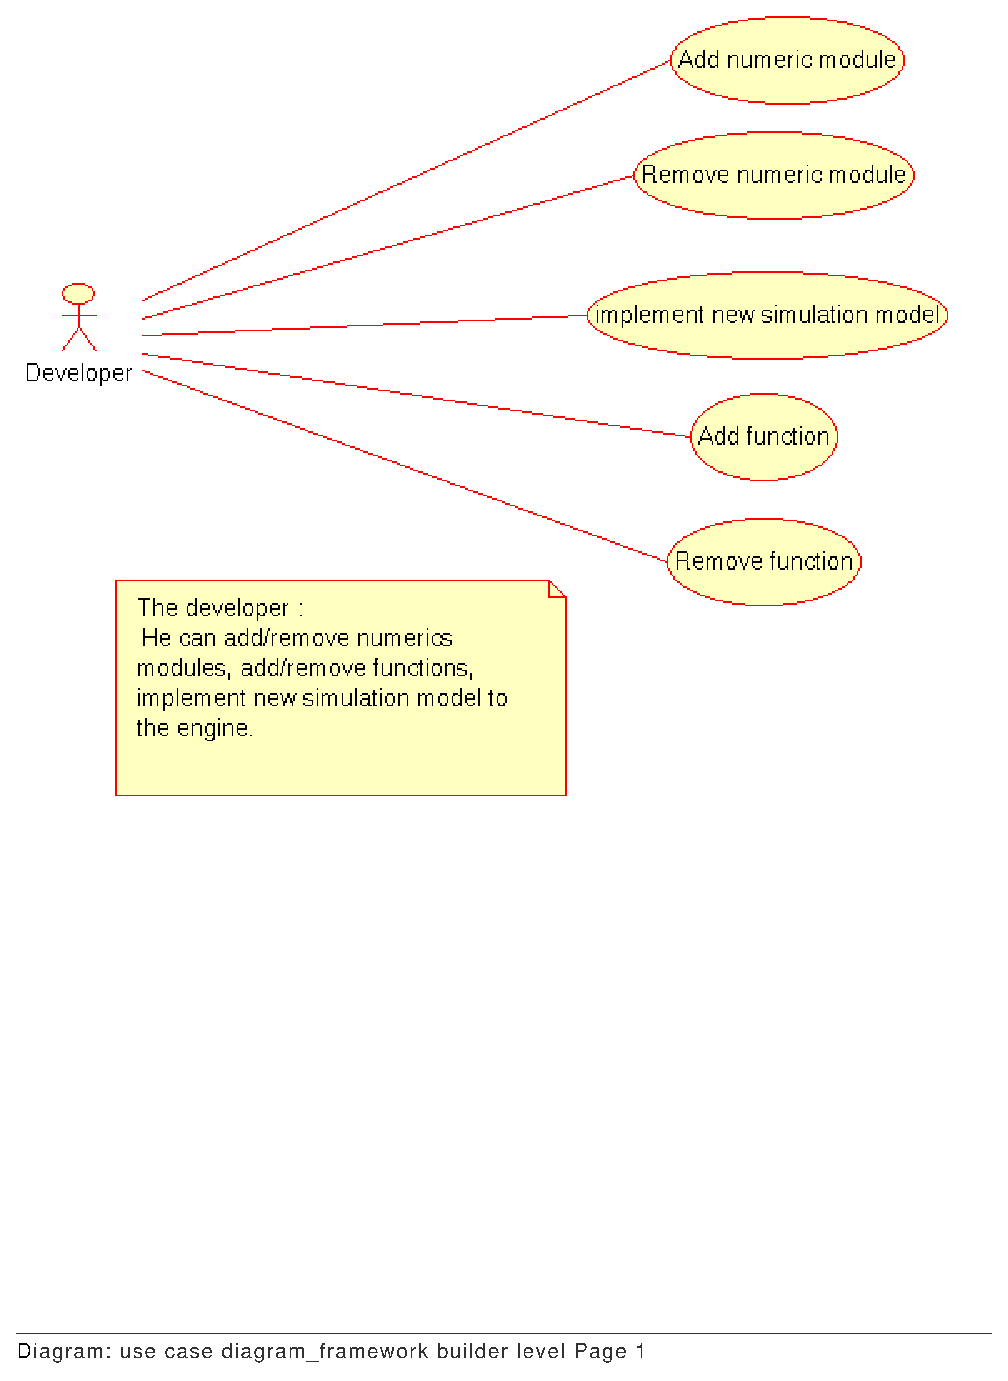
\includegraphics[scale=0.65, bb=0 300 540 700, clip]{figure/use_case_developer_user.eps}
  \end{center}
  \caption{Use case diagram - Developer}
  \label{Fig:Use case diagram - Developer}
\end{figure}

\clearpage

% ----------------      sub-section             ----------------------------------------------------%
\subsection{Users use case}
This case shows how the users can take advantage of the software to run a simulation (see Figure \ref{Fig:Use case diagram - User}).
\begin{figure}[hb]
  \begin{center}
    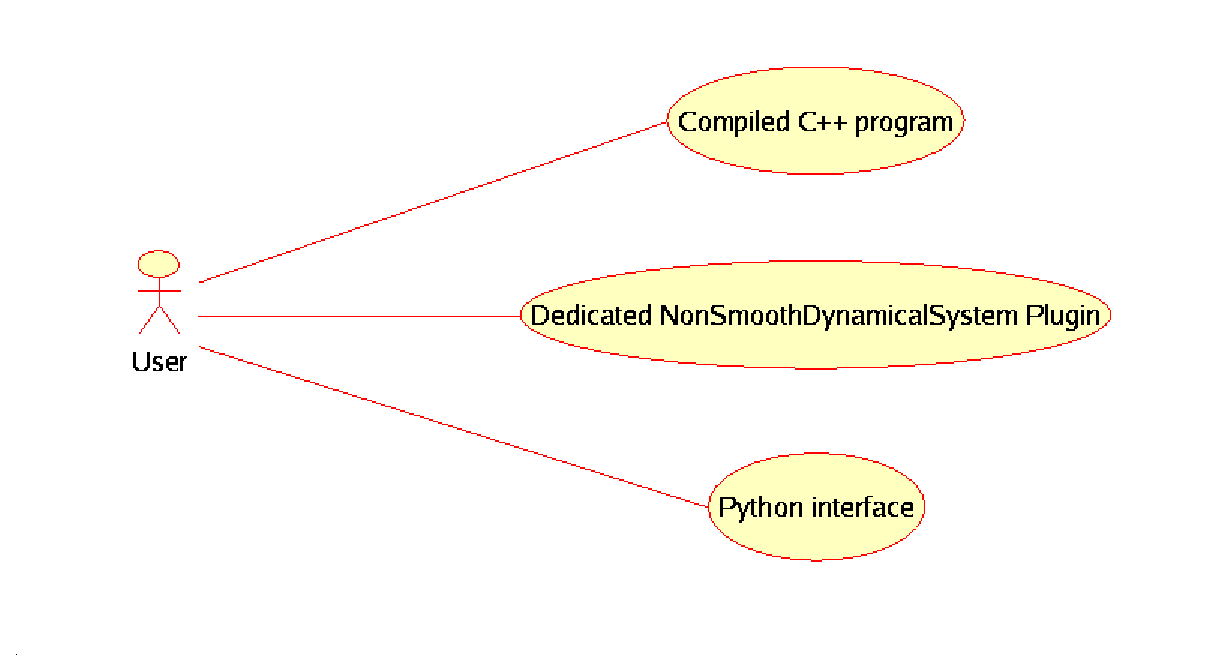
\includegraphics[scale=0.65, clip]{figure/use_case_user.eps}
  \end{center}
  \caption{Use case diagram - User}
  \label{Fig:Use case diagram - User}
\end{figure}

% ----------------      sub-section             ----------------------------------------------------%
\subsection{Scenarii}
These are some examples of scenarii in accordance with every users and their using contexts :
\subsubsection{End user}
\begin{itemize}
\item Mr Chabrier runs \ac{scilab} to invoke the \ac{siconos} platform for a new  simulation. He has already input files in \ac{lmgc90} format defining the problem and its initial state. Its \ac{siconos} input data are defining  the kind of mathematical model and numerical strategy, the engine will use. Mr Chabrier specifies he wishes to save the results at the end of the simulation. Then he can carry out his simulation.
\item Mr Chabrier runs \ac{scilab} to invoke the \ac{siconos} platform for a new  simulation. In this case, he provides several \ac{siconos}  data files in \ac{xml} format, which define completely the problem.  Mr Chabrier also decides  that the outputs of the simulation will be made every "10 time step" during the computations, and to extract, at every time step, the coordinates of an object. Then he can carry out his simulation.
\item Mr Chabrier runs \ac{scilab} to invoke the \ac{siconos} platform for a new  simulation. He uses \ac{scilab} to define all the data (matrices, functions, scalar parameters, \ldots). Then he can carry out his simulation.
\end{itemize}

\subsubsection{Expert user}
\begin{itemize}
\item Mr St Saens is not satisfied by the existing numerical models in the platform. He needs a new one and decides to create it. Using the functionalities given by the platform, he plugs  a new external functionality. This new functionality is invoked through the  C++ interpretor.  He has the \ac{xml} input files and he wants only the final result. Once he has defined some additional parameters, he can carry out his simulation.
\end{itemize}

\subsubsection{Developer}
\begin{itemize}
\item Mr Ravel knows Mr St Saens. Mr St Saens asked Mr Ravel to implement the new functionality, he has developed and tested carefully. Mr Ravel inserts the St Saens' code into the engine and make all the modifications needed by this operation. As a consequence, everybody can use the new functionality in downloading the new version of \ac{siconos}.
\end{itemize}

% ---------------------------------------------------------------------------------------%
% %
% CHAPTER                                                                                                                               %
% %
% ---------------------------------------------------------------------------------------%

\chapter{Interfaces of the software}

This chapter deals with the interfaces of the platform. Two types of interfaces are planned, the first one is a ``command-line'' interface given by \ac{frontend}. The other one will be a graphical one included in \ac{prepost}.

% ---------------------------------------------------------------------------------------%
% section                                                                               %
% ---------------------------------------------------------------------------------------%
\section{The module \acs{frontend}}

% ----------------      sub-section             ----------------------------------------------------%
\subsection{\acs{api} C++ }

This so called \acs{api} C++ will contain :
\begin{itemize}
\item All of the public methods or functions of the \acs{engine}
\item An additional set of high level C++ methods in order to provide a macro language to drive the platform. 
\end{itemize}

This API could be used in two different ways :
\begin{itemize}
\item Compiled directly in an other application or a main file
\item Python interface based on the C++ \ac{api}
\end{itemize}

% ----------------      sub-section             ----------------------------------------------------%
\subsection{\acs{api} for \ac{xxxlab}}

This \acs{api} will interface the high level methods of the platform to allow the command of the platform trough \ac{xxxlab}.

% ---------------------------------------------------------------------------------------%
% section                                                                               %
% ---------------------------------------------------------------------------------------%
\section{The module \acs{imse}}

The contents of this module is not yet defined. The key idea is to develop a graphical user interface based on the \ac{engine}. This graphical user interface will provide a modeling and a visualization environment for the \ac{siconos} platform.


% ---------------------------------------------------------------------------------------%
% %
% CHAPTER                                                                                                                               %
% %
% ---------------------------------------------------------------------------------------%

\chapter{Input and output data}

% ---------------------------------------------------------------------------------------%
% section                                                                               %
% ---------------------------------------------------------------------------------------%
\section{Input data}

The \ac{nsds} which is simulated is completely defined by the input data. As it is explained in the \ac{srd}, there are 3 ways to inform the internal data structure :
\begin{itemize}
\item The complete representation of the problem is loaded by reading \ac{siconos} specific and self-contained files. This way corresponds to a stand alone use of the platform.These files should be \acs{xml} files. 
\item The complete representation of the problem is loaded partially by reading \ac{siconos} specific files. In order to complete the missing part, the user has to provide the information using the API in interactive mode (python interface or the \ac{xxxlab} interface).
\item The complete representation of the problem is given by mixed files : external files describing the physical problem and its state and \ac{siconos} specific files describing the  model formalization and the numerical strategy. This way corresponds to a mixed use of the platform, in combination with an external software.
\end{itemize}

\subsection{End user input data}
The end user will use only XML input files to give data to the platform. That's the easiest way to use the software.
This user must fill all the fields of the XML file structure to specify the formalization of his dynamic systems and the strategy to make
computations.

\subsection{Expert user input data}
An expert user will be able too to give the platform's data by using the methods of the \ac{api} to build the objects required for the
computations with consistant information. He can also use an XML input file and then adding/changing data with the methods of the
\ac{api}.

% ---------------------------------------------------------------------------------------%
% section                                                                               %
% ---------------------------------------------------------------------------------------%
\section{Output data}

Two types of output data for the \ac{engine} may be defined: the output on the standard output and the output in specific data files.

% ----------------      sub-section             ----------------------------------------------------%
\subsection{Standard output}
On the standard output (screen or log file), the user will find some information about the unfolding of the simulation. Particularly, each functions of the \ac{api} could write informations on the standard output during the simulation. The users will choose the verbose level (all informations on the screen, some messages or none).

% ----------------      sub-section             ----------------------------------------------------%
\subsection{Output data files}
Two types of output in the output data files are required:
\begin{itemize}
\item \textbf{Final or intermediate results} \\
  At every moment, during or at the end of the simulation, all the data of the platform can be stored in an \ac{xml} file. That's the user who decides when he wants to save the data (for example, each $n$ steps of simulation).\\
  The information stored are allowing to restart the simulation, it must contain all required data to continue the computations from the state of the last time step saved.\\
  The \ac{xml} files dedicated to the storage of the simulation's data are not overwritten. So at the end of the computations, several output files have been created and can be used to understand the results of the simulation.
  % These results are stored in output data files with a given frequency (at every $n$ steps of simulation). This output data file will be overwritten when a new storage is made. Perhaps, two increments may be saved for safety reasons. The storage of these results at the end of the simulation is a particular case  of the intermediate results. The goal of this type of results is to ensure a restart of a simulation and a complete backup of the state of the platform. These output data files must contain all of the informations required to restart a simulation at a given step.  A structured file (by example an \acs{xml} file) which describe clearly the formalized model, the numerical simulator and the objects of the simulation must contain this information. The structure of the initial input file and of a intermediate file  must be the same in order to restart a simulation just by a copy of this file.

\item \textbf{Partial results} \\
  They are data stored during the computations with a given sequence in output data files. That's the user who have to select the data he wants to save and to manage the file writing. Saved file are not necessary \ac{xml} files, the user decides how he wants to store the information. For example, the user can save in a simple ascii file the speed of each dynamical system of his system, at each time steps.\\
  % Partial results are data, stored during the computations with a given sequence in an other output data files. Contrary to the previous case, only partial results are stored but all of the history of these results are conserved all along the simulation to allow the user to study the evolution of these results during the simulation. In this case, the user has to define the  results, he want to save and the frequency of the storage.

\end{itemize}


% ---------------------------------------------------------------------------------------%
% %
% CHAPTER                                                                                                                               %
% %
% ---------------------------------------------------------------------------------------%

\chapter{Basics errors}
There are two main types of errors in the platform. In one hand, the input data can be erroneous. In the other hand, users can make mistakes when they use an interface. The internationalization imposes us to write error messages in severals languages. So will have to use structured files to store the error messages.\\
Each error message must explain when and why it appears.

% ---------------------------------------------------------------------------------------%
% section                                                                               %
% ---------------------------------------------------------------------------------------%
\section{Input files errors}
The input file can be an \ac{xml} file, or a plugin.
\begin{itemize}
\item Fail to open input files
\item Missing input file(s)
\item Invalid structure of an input file
\end{itemize}

% ---------------------------------------------------------------------------------------%
% section                                                                               %
% ---------------------------------------------------------------------------------------%
\section{Input users errors}
\begin{itemize}
\item Invalid input data
\item Incorrect use of function
\item Wrong or bad parameters of a function
\end{itemize}

% ---------------------------------------------------------------------------------------%
% section                                                                               %
% ---------------------------------------------------------------------------------------%
\section{Errors during the computations}
If the simulation abort during the computations, errors messages must help to determine where and why a failure occurs. It will be important to give error messages which will be clear and concise. These errors can be mathematical errors (division by 0, matrix dimensions incompatible, \dots) or errors if the program trys to read a data which not exists (trying to access an element in a vector with an index greater than the vector size, \dots).
\pagestyle{empty}

% \printglosstex(glo)[p]
\printglosstex(acr)[p]
\cleardoublepage
\end{document}
